
% % \paragraph{Sơ đồ tuần tự Luồng Hội thoại giọng nói}

% % Luồng nghiệp vụ này mô tả Hội thoại giọng nói theo thời gian thực giữa người dùng và AI Voice Agent, bao gồm từ bước cấp quyền, thiết lập phòng họp LiveKit, đến quá trình xử lý ngôn ngữ, tra cứu RAG pháp luật và phản hồi âm thanh (TTS).

% % \begin{figure}[H]
% % \centering
% % 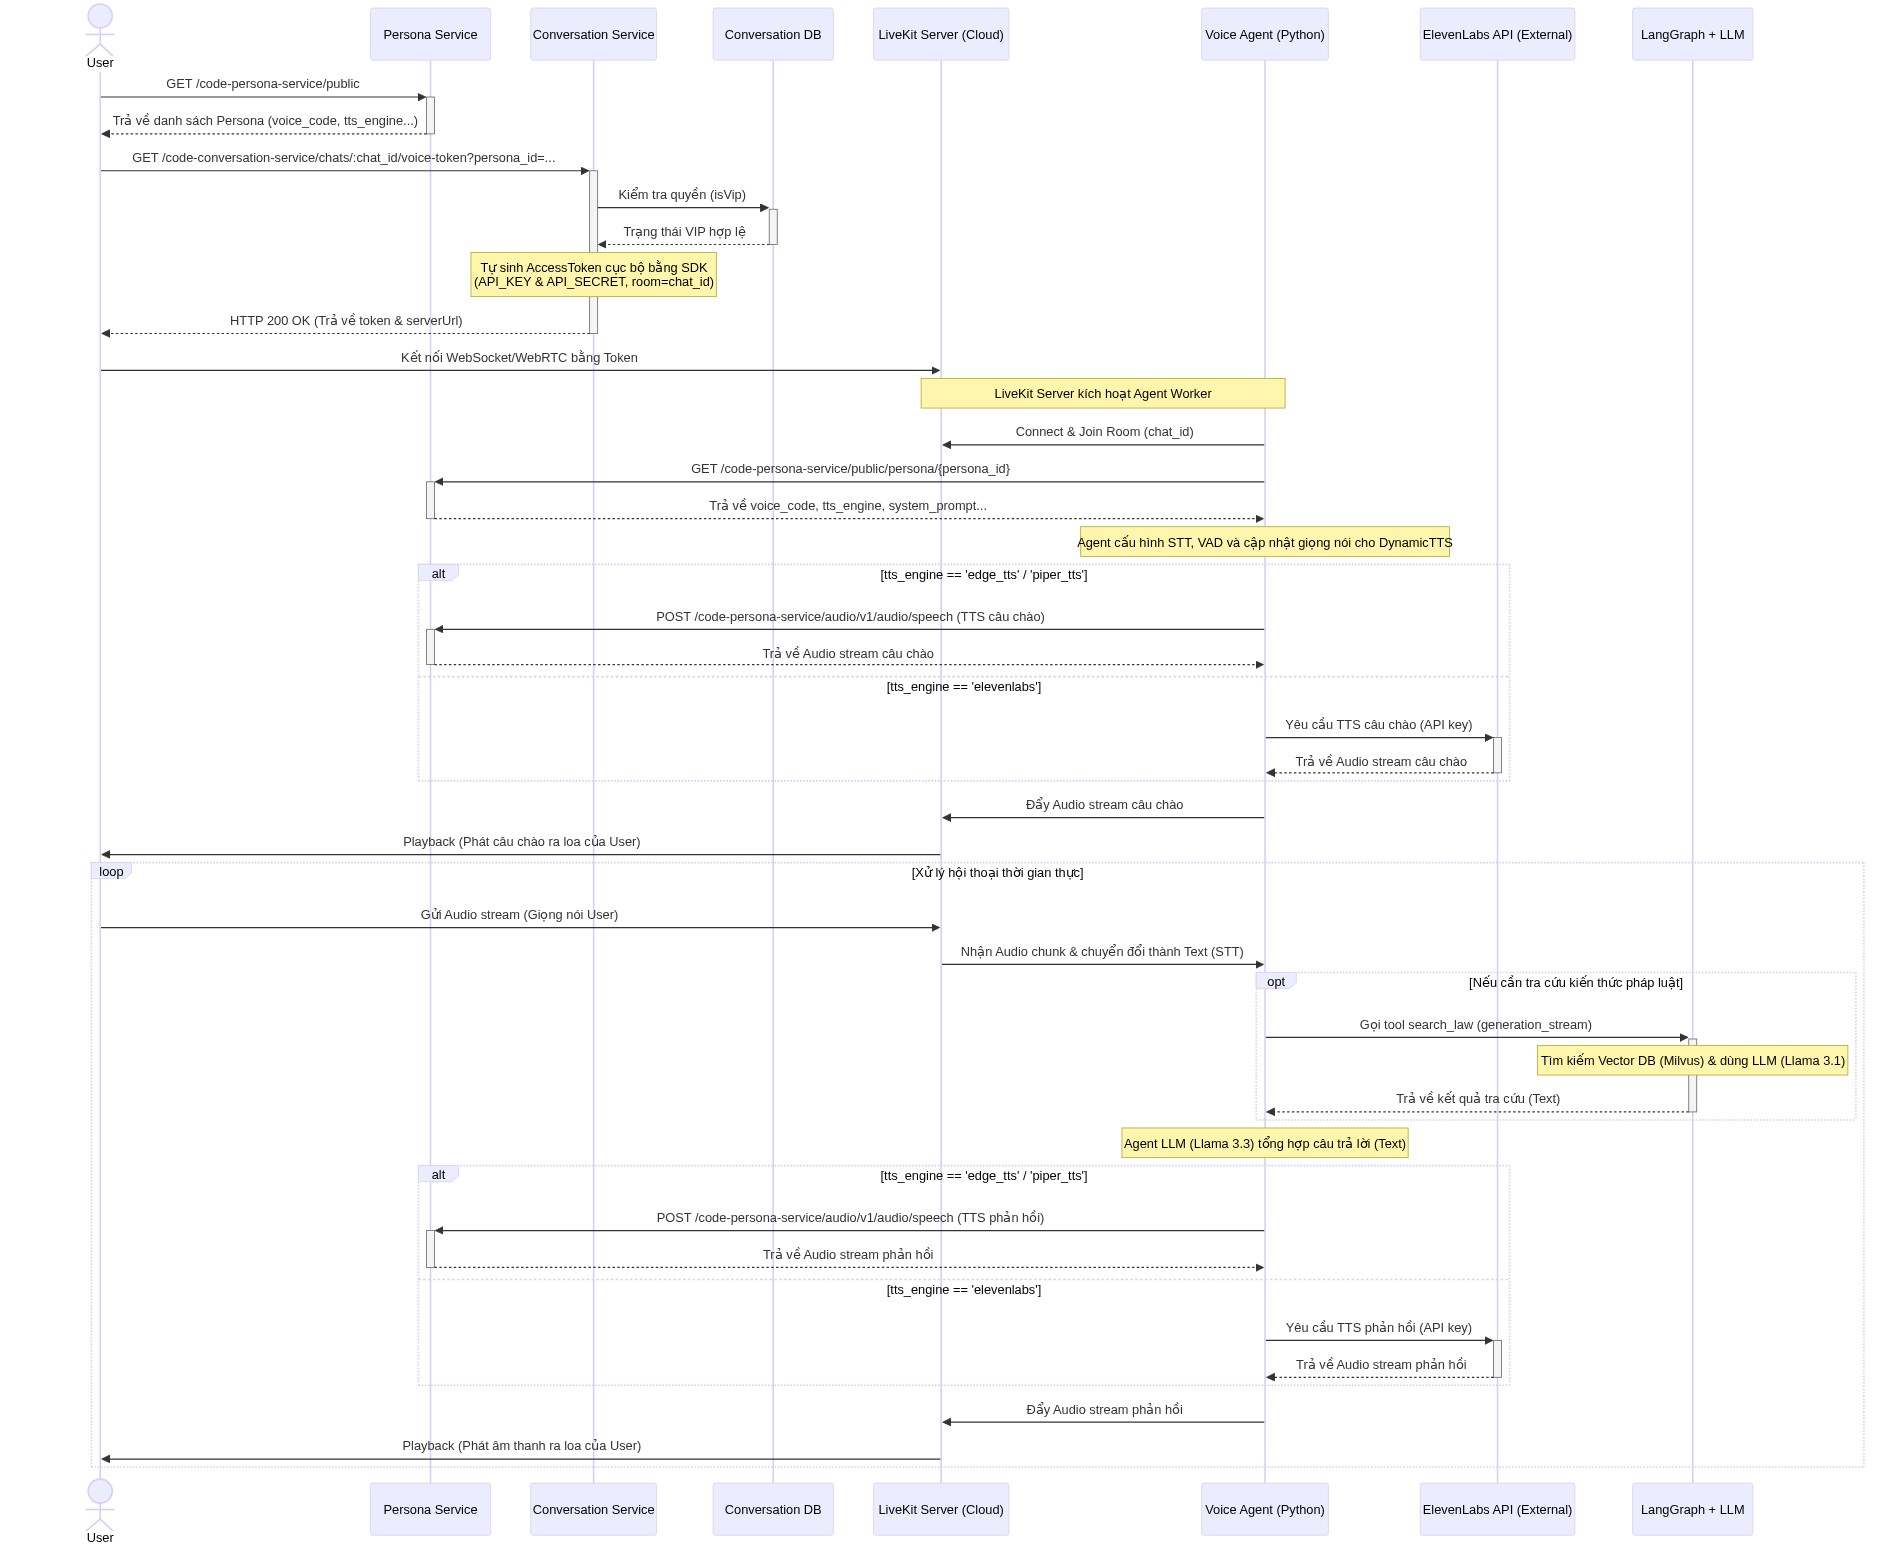
\includegraphics[scale = 0.18]{pictures/Sequence-voice.png}
% % \caption{Sơ đồ tuần tự Luồng Hội thoại giọng nói}
% % \end{figure}

% % \subparagraph{Các thành phần tham gia}

% % \begin{table}[H]
% % \centering
% % \renewcommand{\arraystretch}{1.3}
% % \begin{tabular}{|l|l|p{5cm}|}
% % \hline
% % \textbf{Thành phần} & \textbf{Phân loại} & \textbf{Vai trò trong hệ thống} \\ \hline
% % User & Actor & Người dùng thực hiện thao tác tương tác bằng giọng nói. \\ \hline
% % Persona Service & Microservice & Quản lý thông tin của nhân vật và đảm nhiệm sinh giọng nói (edge\_tts, piper\_tts). \\ \hline
% % Conversation Service & Microservice & Xử lý tạo phiên trò chuyện, kiểm tra quyền người dùng và cấp phát Access Token cục bộ cho dịch vụ LiveKit. \\ \hline
% % Conversation DB & Database & Lưu trữ dữ liệu phiên chat và thông tin người dùng bảng UserSubscription. \\ \hline
% % LiveKit Server & Cloud Service / WebRTC & Máy chủ trung gian xử lý các kết nối WebRTC, phân phối và truyền phát luồng dữ liệu giữa User và Agent. \\ \hline
% % Voice Agent & Agent & Đảm nhiệm điều phối trò chuyện, sử dụng LangGraph. \\ \hline
% % ElevenLabs API & External Service & Nền tảng bên thứ ba cung cấp dịch vụ TTS. \\ \hline
% % LangGraph + LLM & AI Engine & Xử lý ngôn ngữ tự nhiên, tạo chuỗi suy luận và sinh văn bản phản hồi. \\ \hline
% % \end{tabular}
% % \caption{Danh sách các thành phần và vai trò trong Sơ đồ tuần tự Luồng Hội thoại giọng nói}
% % \label{tab:system_components_voice}
% % \end{table}

% % \subparagraph{Mô tả tổng quan}

% % \begin{itemize}
% % \item Người dùng gọi API lấy cấu hình nhân vật hiện có và yêu cầu Voice Token cho chat\_id cụ thể.
% % \item Dịch vụ trò chuyện kiểm tra điều kiện bảng UserSubscription.
% % \item Dịch vụ trò chuyện tạo Access Token LiveKit cho người dùng.
% % \item Người dùng sử dụng Token để kết nối WebRTC tới LiveKit Server.
% % \item Voice Agent tham gia vào cùng phòng người dùng.
% % \item Voice Agent lấy thông tin nhân vật và cấu hình giọng nói (Persona Service hoặc ElevenLabs).
% % \item Voice Agent chủ động chào hỏi người dùng.
% % \item Voice Agent sử dụng LangGraph tạo câu trả lời và xử lý cuộc trò chuyện với người dùng.
% % \end{itemize}
